\documentclass[letterpaper,11pt]{article}
\usepackage{graphicx}
\usepackage[margin=0.9in]{geometry}
\usepackage{tabularx}
\usepackage{amsmath}
\usepackage{enumerate}
\usepackage{hyperref}
\usepackage{verbatim}
\usepackage{color}
\usepackage{enumitem}


\renewcommand{\vec}[1]{\mathbf{#1}} % Display vectors as boldface %

\let\oldhat\hat   % Also display hats as boldface
\renewcommand{\hat}[1]{\oldhat{\mathbf{#1}}} % Also display hats as boldface

\begin{document}

\title{Update on Time Resolved X-Ray Diffraction Codes}
\author{Eric Landahl}
%\date{}

\maketitle

\section{About this document}
This is a summary of current progress on the TRXD code written and maintained by Eric Landahl, with considerable help from Sooheyong Lee and G. Jackson Williams.  This document will update regularly.

\section{Purpose of the Codes}
\begin{enumerate}
\item{Rocking curve calculations are benchmarked against established codes where possible as well as analytical solutions}
\item{Written entirely in MatLAB}
\begin{itemize}
\item{Compiling not required}
\item{Runs on multiple operating systems}
\item{Octave compatible}
\item{Student friendly}
\end{itemize}
\item{Documented, evolving, and can be used and adapted by others}
\begin{itemize}
\item{Maintained on GitHub and updated regularly}
\item{Revision control and branching is used for development}
\item{Extensive comments, manuals, and benchmarks included with distribution}
\end{itemize}
\item{Efficient and flexible operation}
\begin{itemize}
\item{Extensive use of remeshing: the spatiotemporal grid for electron diffussion, thermal diffussion, acoustic propagation, and diffraction calculations do not need to be the same, or even have evenly spaced steps}
\item{Adaptive step sizes in the diffraction algorithim allow speed and accuracy to be tuned}
\item{Vectorization and boolean indexing are used for speed and are parallel computing compatible}
\end{itemize}
\item{Multiple crystals and x-ray energies}
\begin{itemize}
\item{Presently focusing on 7 - 14 keV, Ge, GaAs, Si, and InSb symmetric 004 reflection}
\item{Distribution includes self contained diffraction parameter (e.g. $\chi$) database}
\end{itemize}
\item{Easy to develop strain functions}
\begin{itemize}
\item{Distribution includes database of common material properties (e.g. sound velocities, specific heat, etc.)}
\end{itemize}
\end{enumerate}

\section{Dynamical diffraction calculations: \\Issues with implementation of the Wie et al. algorithm}

There are a lot of problems in taking a nearly 25 year old paper designed to calculate x-ray diffraction from multilayers and superlattices and apply it to continuously varying strain parameters.  In this section I will be trying to clean up and solve some issues that have plagued the implementations of this algorithm by the time-resolved x-ray community.  For now I will just briefly list some of the issues.

\subsection{Substrate boundary condition}
The iterative solution proposed by Wie et al. relies on an unstrained semi-infinite crystal being present below the strained layers.  This means that the strain must approach zero before the calculation begins.  Jackson suggested multiplying the strain by

\begin{equation}
e^{-z/L_{ext}}
\end{equation}
where $z$ is the depth below the surface and $L_{ext}$ is the extinction length.  This tapers off the large impulsive acoustic strains that travel deep into the crystal, which otherwise would at some timepoints violate the zero-strain boundary condition.  The problem with this approach is that the tapering is too severe.  Specifically for thermal transport problems, where the shape of the strain profile is being studied over several microns, this tapering alters the outcome of the rocking curve calculation.  This implementation instead uses a deeper strain tapering function,
\begin{equation}
 \frac{1-erf\left(\frac{2z}{L_{ext}} - 8\right)}{2}.
\end{equation}
A consequence of this new taper function (see Fig.\ref{fig:taper_fig}) is that the calculation must begin much deeper.  The code checks to make sure that the given strain profile is at least $5L_{ext}$ deep, and begins calculations just inside of this point, where the strain is therefore forced to be zero.  

\begin{figure}
\begin{centering}
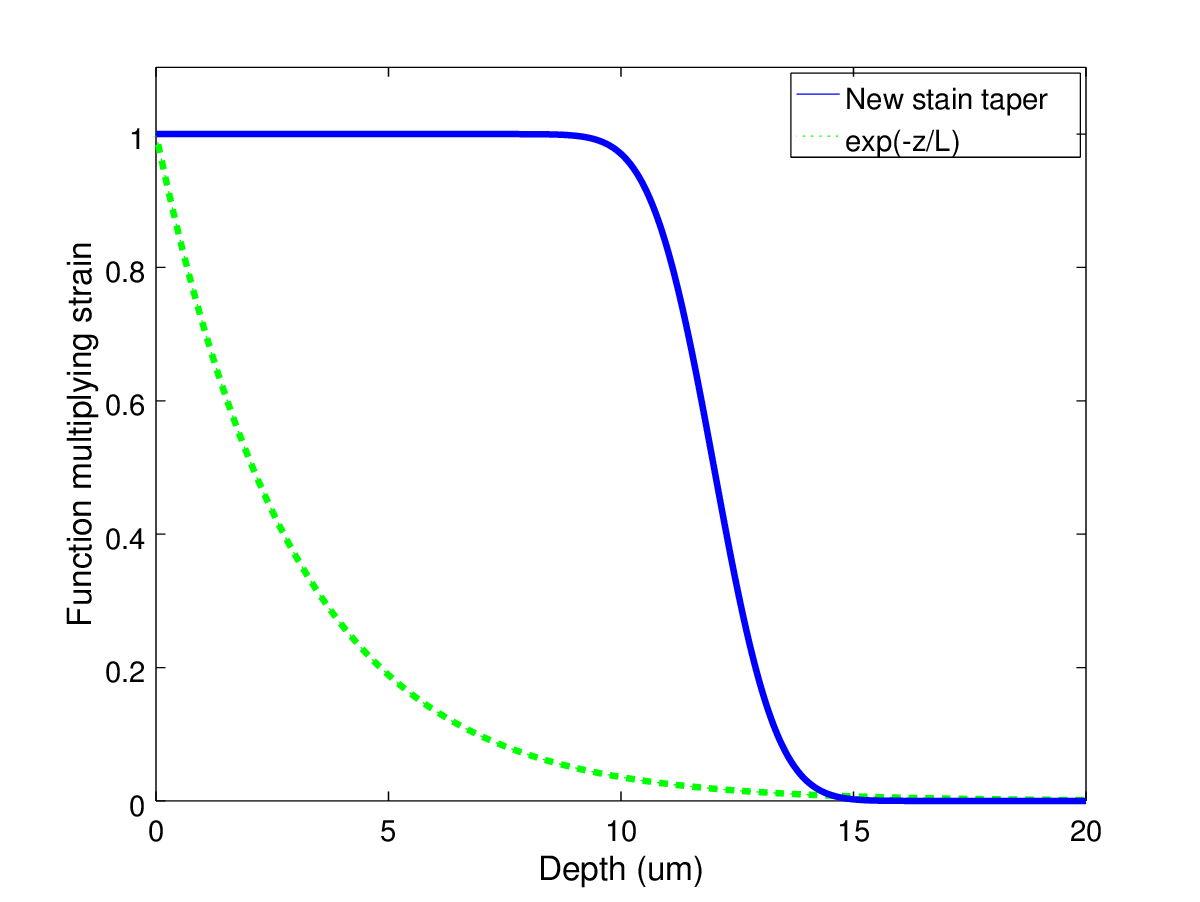
\includegraphics[scale = 0.65]{Taper_functions.png}
\caption{Envelope or taper function applied to depth-dependent strain profile to make sure that the strain is unchanged within several extinction lenths of the surface, but tapers to zero before the calculation begins at $5L_{ext}$.  For this example, an extinction depth of $L_{ext}=3 \mu m$ was used.}
\label{fig:taper_fig}
\end{centering}
\end{figure}

\subsection{Depth step size}
An unfortunate consequence of choosing such a deep starting point is that more iterations of the Wie et al. algorithm are required, if a fixed depth step is used.  This motivates some thought about the choice of the correct depth step.  Wie et al. intended their method to be used for multilayers and superlattices, where the depth step was given by the thickness of a particular layer.  In practice, we have used fixed depth steps, reduced in size until the output result no longer changes.  A better approach for continually variable strain profiles is to use an adaptative step size.  This allows the step size to be changed as the strain varies to maintain a maximum error tolerance.  An adaptative step size algorithm is used in the function \texttt{WieAdapt.m}.  Briefly, a full step is compared to the (presumably more accurate) result for two successive half steps. The difference is compared to a relative error tolerance to determine the next step size.  A plot illustrating the adaptative step size algorithm at will be added to this document soon.  Other more sophisticated adaptative algorithms could be developed. Another option is solving the simplified Tagaki-Taupin equations using an adaptative Ordinary Differential Equation routine (e.g. MatLAB's \texttt{ode45}).  

\subsection{Ambiguity in sign of the square root of an imaginary number}
The Appendix in Wie et al. gives a useful, but somewhat under-developed description of taking the square roots of a complex number.  I have found that for my given choices of the signs of $\chi$ that the following sign choices give the physcally realistic solutions:

\begin{equation}
TBA
\end{equation}
The sign conventions I used for the electric susceptibilities are compared to those of Sergey Stepanov's $\chi_{0h}$ program in Table \ref{table:sign_conventions}.  The signs are adjusted upon input in the program \texttt{TRXD.m}.More work will need to be done to clarify exactly why these particular sign conventions should be used.  

\begin{table}
\begin{centering}
\begin{tabular}{c | c | c}
parameter  & TRXD & $\chi_{0h}$ \\
\hline
$\chi_{0}\prime$ & - & - \\
$\chi_{0}\prime\prime$ & + & + \\
$\chi_{h}\prime$ & - & + \\
$\chi_{h}\prime\prime$ & + & + \\
\end{tabular} 
\caption{Sign conventions for susceptibilities $\chi_{0}=\chi_{0}\prime+i\chi_{0}\prime\prime$ is the susceptibility for the incident beam and $\chi_{h}=\chi_{h}\prime+i\chi_{h}\prime\prime$ is the susceptibility for the diffracted beam.}
\label{table:sign_conventions}
\end{centering}
\end{table}

\subsection{Normalized depth}
The biggest challenge, and the one not completely resolved is the proper choice of normalized length scale $A$.  The definitiion given by Wie et al. does not appear to aggree with either analytical models or GID-SL.  I have implmented a linear correction in $sin(\theta_B)$ that returns the proper values for GaAs from 8 - 11 keV.  Extending to other crystals and a wider energy range should be possible with a higher-order, empirical correction.  This area definitely needs further study.  

\section{User's Manual}
The manual still needs to be written.  In the meantime, the best way to access the codes is to run the simple script \texttt{TRXD\_Driver\_example.m}.  Table \ref{table:codeparams} gives a summary of some parameters that can be easily adjusted by the user.

\begin{table}
\begin{centering}
\begin{tabular}{c | l | c}
line number  & variable & description \\
\hline
19 & \texttt{energy} & x-ray energy in keV \\
16 & \texttt{crystal} & 'GaAs', 'Ge', 'InSb', or 'Si' \\
20 & \texttt{fluence} & in mJ/cm$^2$, or timepoint number \\
15 & \texttt{model} & see next section \\
81 & \texttt{plot\_opts} & 'none' or 'final' \\
82 & \texttt{angle\_res} & blurs plots, only used for full 2D calcs \\
\end{tabular} 
\caption{Parameters that can be easily set by the user when running the script \texttt{TRXD\_Driver\_example.m}.}
\label{table:codeparams}
\end{centering}
\end{table}

\subsection{Benchmarking against Sergey Stepanov's GID-SL diffraction calculations}
The first step upon downloading the code package should always to use the 'benchmark' method as described in this section.  It is not necessary to run GID-SL, since the standard benchmark file is included in the distribution.  However, to check other crystals, energies, or simple analytic strain models GID-SL can be run from \url{http://x-server.gmca.aps.anl.gov/GID_sl.html}, and then choosing the option for ``Symmetric Bragg diffraction from multilayers and superlattices". The standard benchmark condition is 10 keV, GaAs 004, with a constant strain of $10^{-4}$ over the first 2 $\mu m$ of depth. GID-SL should be set to these parameters, with a single line of code in the textbox specifying the single strained layer as \texttt{t = 20000 code = GaAs da/a = 1E4}.  Note that the thickness units used by GID-SL are in Angstroms.  The anglular range should be set from -0.01 to +0.01 degrees.  Figure \ref{fig:GID-SL} shows a screenshot of how this screen should look. The results should be opened in \texttt{.dat} format and saved as \texttt{/benchmarks/benchmark.txt}.  This file will be automatically plotted alongside the TRXD calculations when the method is chosen to be 'benchmark'.  The standard benchmark conditions are given in Table \ref{table:benchmark}.  The results of running the code should give one logarithmic and one linear scale plot, each with 3 lines corresponding to the unstrained rocking curve, the TRXD calculated strained rocking curve, and the output of GID-SL. \emph{There are still some minor discrepencies between GID-SL and TRXD that are being worked out.}

\begin{figure}
\begin{centering}
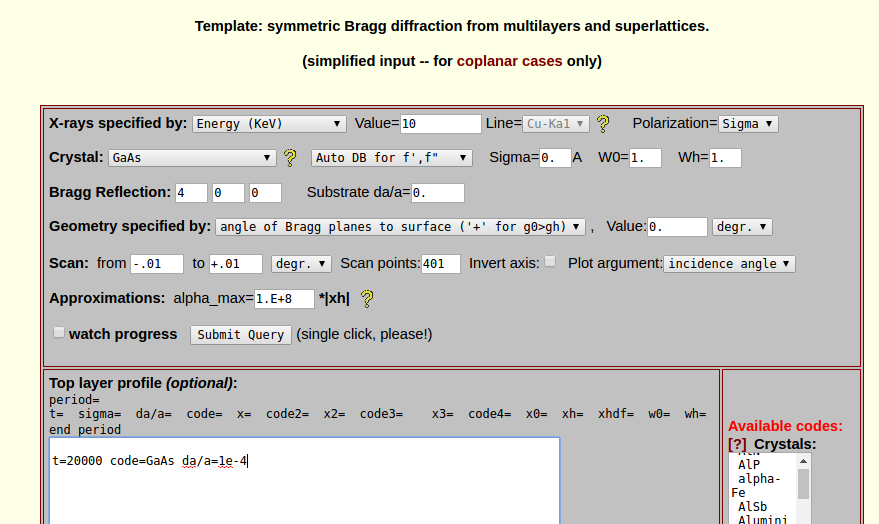
\includegraphics[scale = 0.5]{GID_SL_Benchmark_Screenshot.png}
\caption{Proper configuration of GID-SL to duplicate the standard benchmark results.}
\label{fig:GID-SL}
\end{centering}
\end{figure}

\begin{table}
\begin{centering}
\begin{tabular}{l |c | l | c}
program & line number  & variable & standard benchmark value \\
\hline
\texttt{TRXD\_Driver\_example.m} & 19 & \texttt{energy} & 10 \\
\texttt{TRXD\_Driver\_example.m} & 16 & \texttt{crystal} & 'GaAs' \\
\texttt{TRXD\_Driver\_example.m} & 15 & \texttt{model} & 'benchmark' \\
\texttt{/main/TRXD.m} & 190 & \texttt{longitudinal} & \texttt{=1e-4 * (z<=2e-6);} \\
\end{tabular} 
\caption{Parameters that are used in for comparission with the GID-output file \texttt{/benchmarks/benchmark.txt} included in the distribution.}
\label{table:benchmark}
\end{centering}
\end{table}

\begin{figure}
\begin{centering}
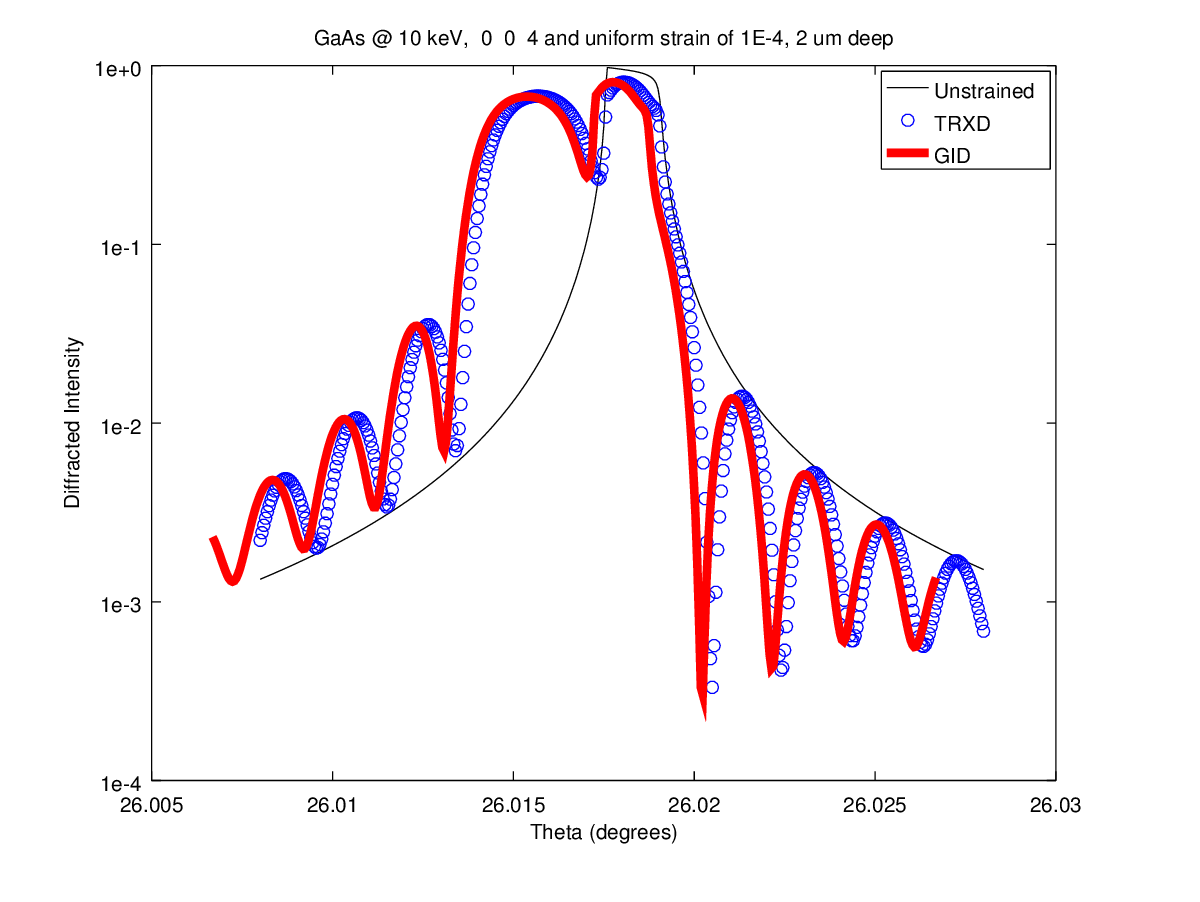
\includegraphics[scale = 0.65]{Log_benchmark.png}
\caption{Results using the configuration given in Table \ref{table:benchmark} and Fig. \ref{fig:GID-SL}.}
\end{centering}
\end{figure}

\begin{figure}
\begin{centering}
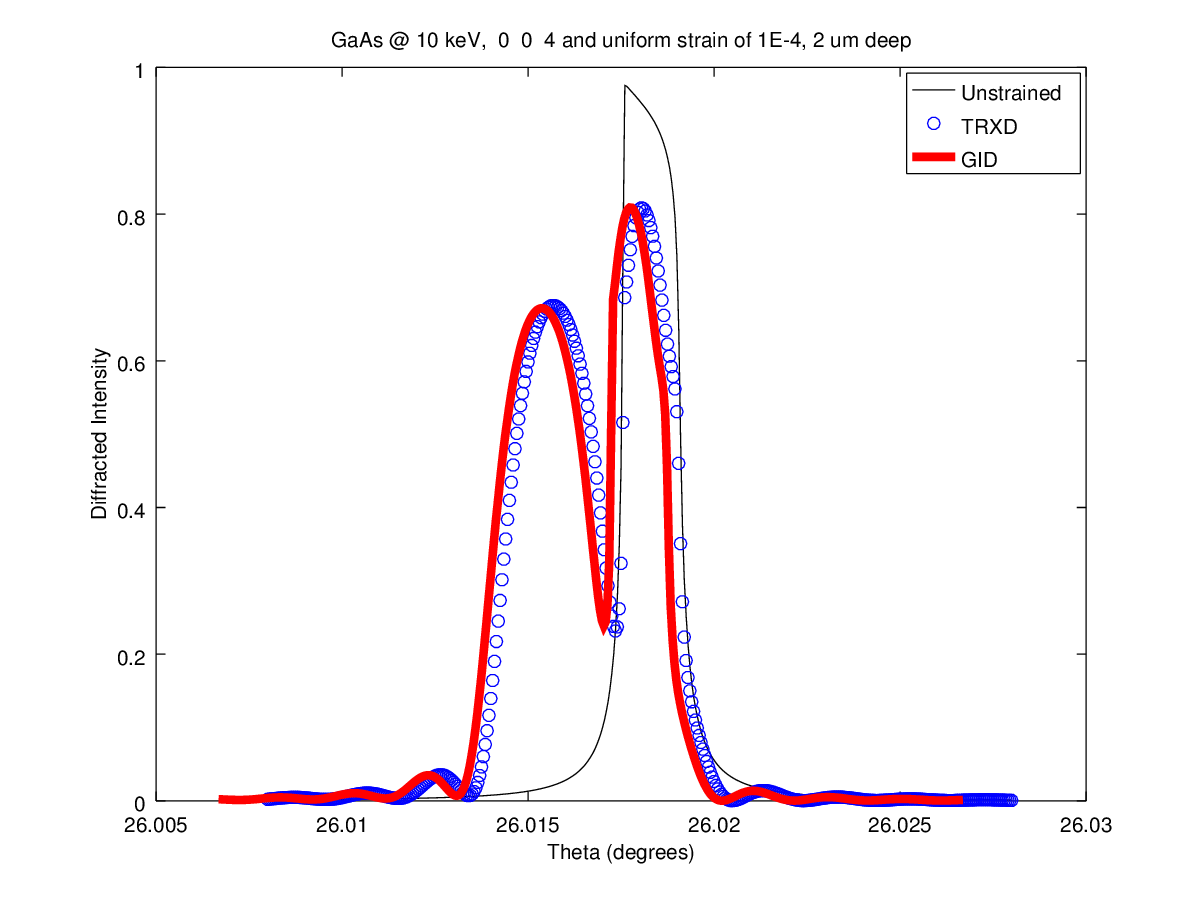
\includegraphics[scale = 0.65]{Linear_benchmark.png}
\caption{Results using the configuration given in Table \ref{table:benchmark} and Fig. \ref{fig:GID-SL}.}
\end{centering}
\end{figure}

\subsection{Testing using an external strain file provided by SHL}
Soo provided a file Soo1.txt containing a previously calculated strain profile.  This strain file was padded with zeros out to 20 $\mu m$ and resaved as \texttt{strain\_file.txt}.  A one dimensional array of times was saved as \texttt{time\_file.txt}, and a one dimensional array of depths was saved as \texttt{depth\_file.txt}. These 3 files will be read anytime the \texttt{model} variable is set to 'strainFile1D' to look at single timepoints.  In this model, the otherwise unused variable \texttt{fluence} is used to set the particular timepoint chosen.  To briefly summarize the provided file, an initially shallow strain genrates a travelling bipolar impulsive wave with a short duration.  As it moves away from the surface, the initial strain profile undergoes diffusion, resulting in a deeper but less dramatic strain.  The \texttt{model} variable can be set to 'strainFile1D' to look at single timepoints.  In this model, the otherwise unused variable \texttt{fluence} is used to set the particular timepoint chosen. 

\begin{figure}
\begin{centering}
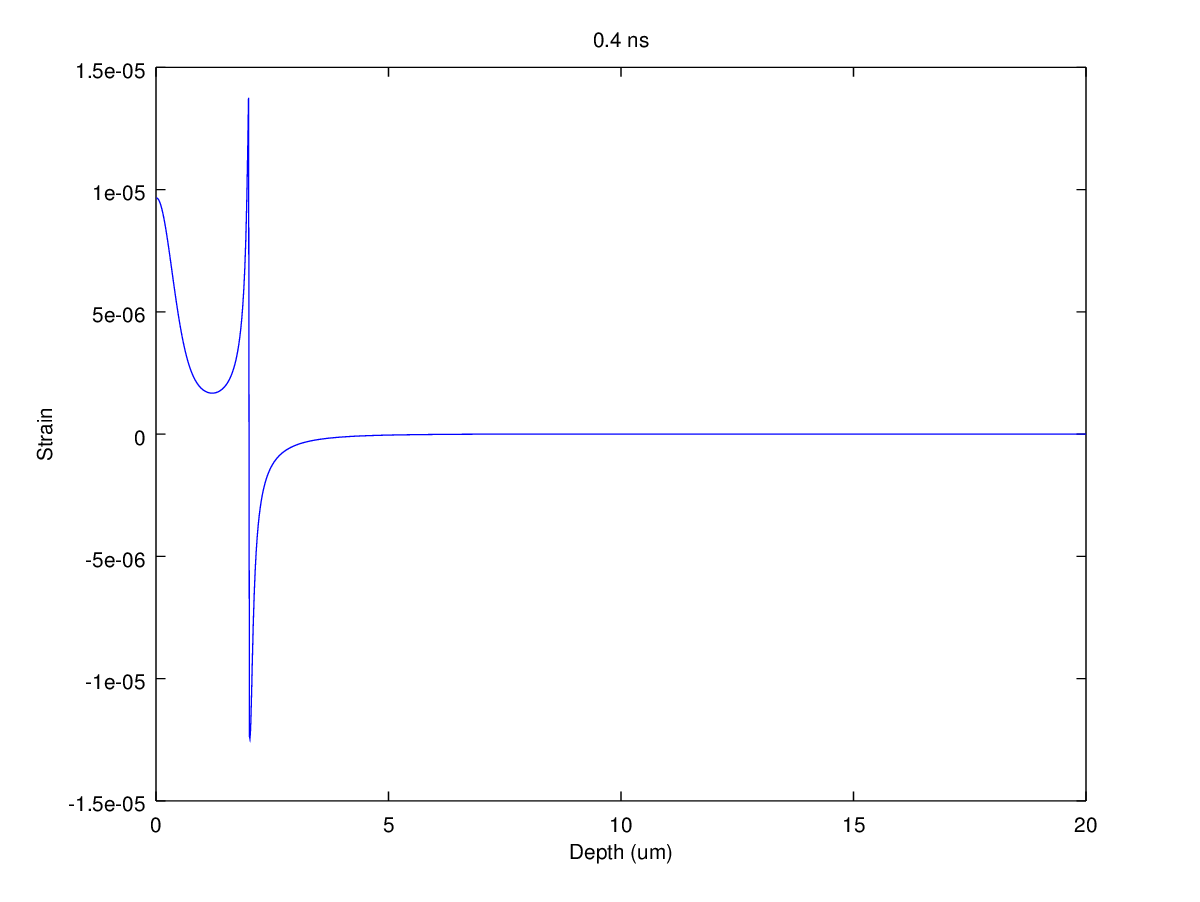
\includegraphics[scale=0.65]{400ps_strain.png}
\caption{External file, 400 ps strain profile.}
\label{fig:400ps_strain}
\end{centering}
\end{figure}

\begin{figure}
\begin{centering}
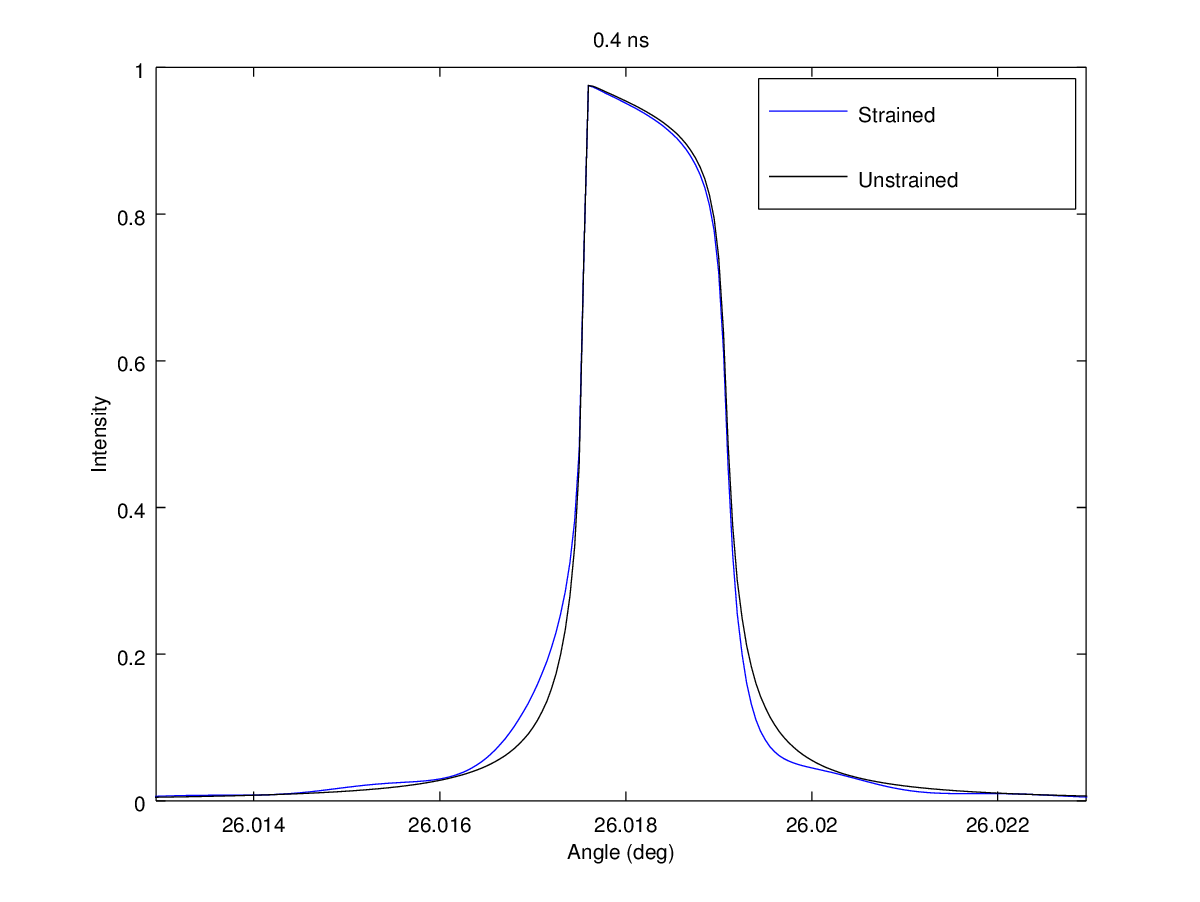
\includegraphics[scale=0.65]{400ps_lin.png}
\caption{External file, 400 ps rocking curve (linear scale).}
\label{fig:400ps_lin}
\end{centering}
\end{figure}

\begin{figure}
\begin{centering}
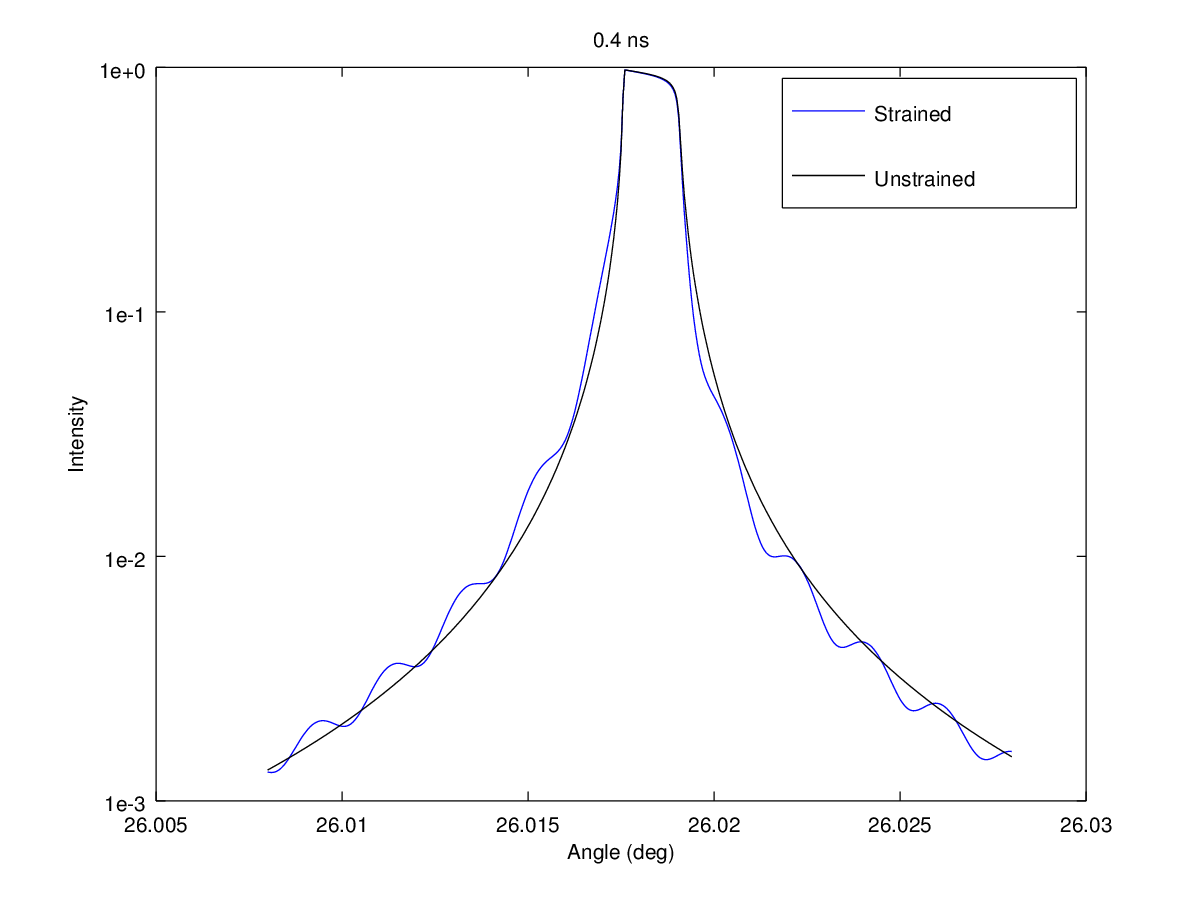
\includegraphics[scale=0.65]{400ps_log.png}
\caption{External file, 400 ps rocking curve (logarithmic scale).}
\label{fig:400ps_log}
\end{centering}
\end{figure}

To demonstrate the validity of the code, I have chosen two timepoints and run them for GaAs 004 10 keV.  The first is 400 ps (200th timepoint).  The strain is shown in Fig. \ref{fig:400ps_strain}.  The strain is confined to about 2 $\mu m$ of the surface.  The rocking curves for strained and unstrained crystal are shown in Figs. \ref{fig:400ps_lin} and \ref{fig:400ps_log}.  As expected, the x-ray diffraction pattern shows a slight shift and considerable modulation fringes.  Both can be analized. The average strain is calculated using the differential Bragg formula, 
\begin{equation}
\dfrac{\Delta d}{d} = -\Delta \theta \: cot(\theta_B)
\end{equation}
whre $d$ is the lattice plane separation, $\Delta d$ is the change in lattice parameter, $\Delta \theta$ is the peak centroid shift determined from the two rocking curves, and $\theta_B$ is the Bragg angle.  The program uses this formulat to produce the following output at 400 ps:  

\medskip
\noindent
\texttt{The centroid shift is -0.086 mdeg or -1.5e-06 radians. For GaAs 0 0 4 at 10.0 keV the estimated average strain is 3.1e-06 .}
\medskip

From inspection of Fig. \ref{fig:400ps_strain}, 3.1e-06 is a reasonable estimate for the average strain in the first few microns.  The fringe spacing can be analyzed to determine the thickness of the strained layer using

\begin{equation}
t = d \dfrac{\theta_B}{\delta \theta_{fringe}}
\end{equation}
where $t$ is the thickness of the strained layer and $\delta \theta_{fringe}$ is the fringe separation angle.  It is easiest to determine the fringe spacing from the logarithmic plot (Fig. \ref{fig:400ps_log}).  For the 400 ps data, the finge spacing is 2 mdeg, and for the GaAs 004 reflection the lattice spacing $d$ = 0.14133 nm.  This calculation yields a strain layer depth $t$ = 1.837 $\mu m$, very close to inspection of Fig. \ref{fig:400ps_strain}.

\begin{figure}
\begin{centering}
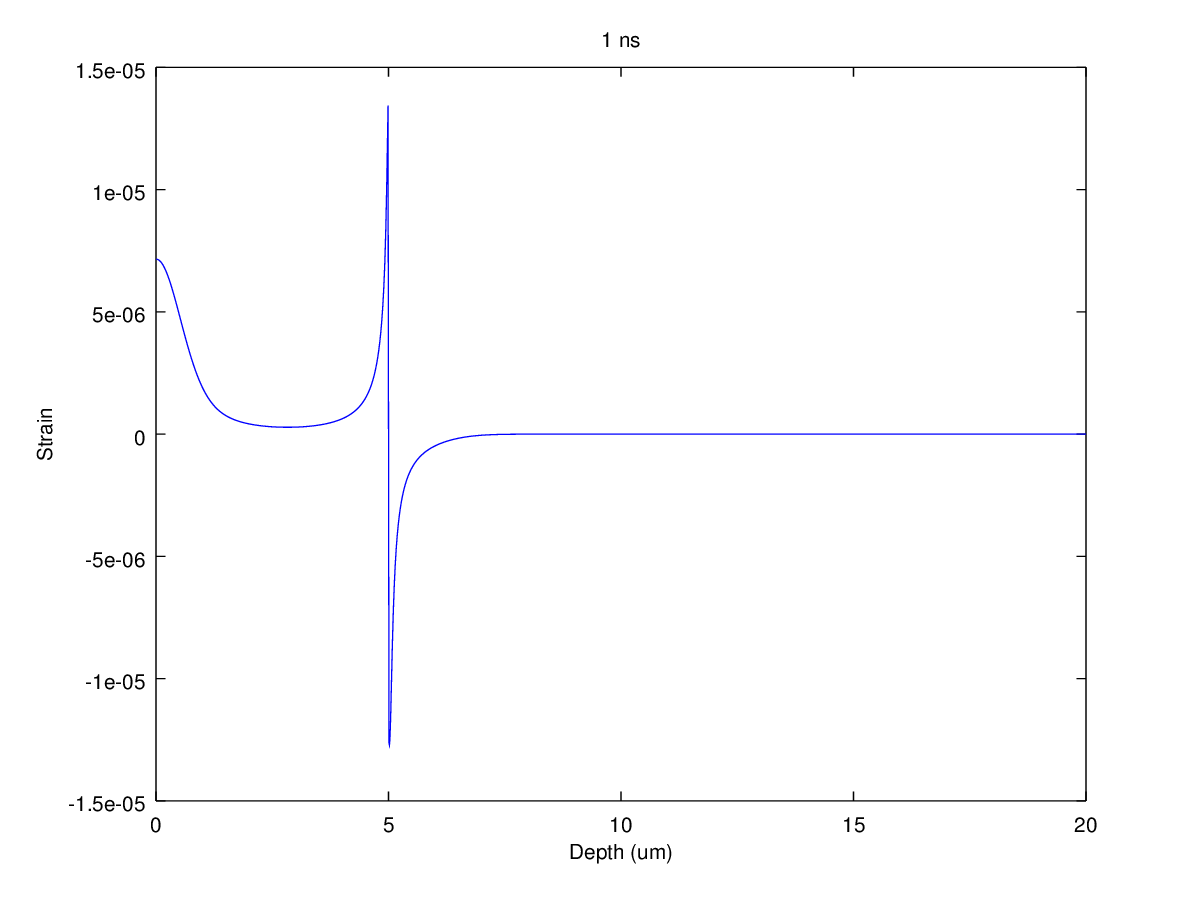
\includegraphics[scale=0.65]{1ns_strain.png}
\caption{External file, 1 ns strain profile.}
\label{fig:1ns_strain}
\end{centering}
\end{figure}

\begin{figure}
\begin{centering}
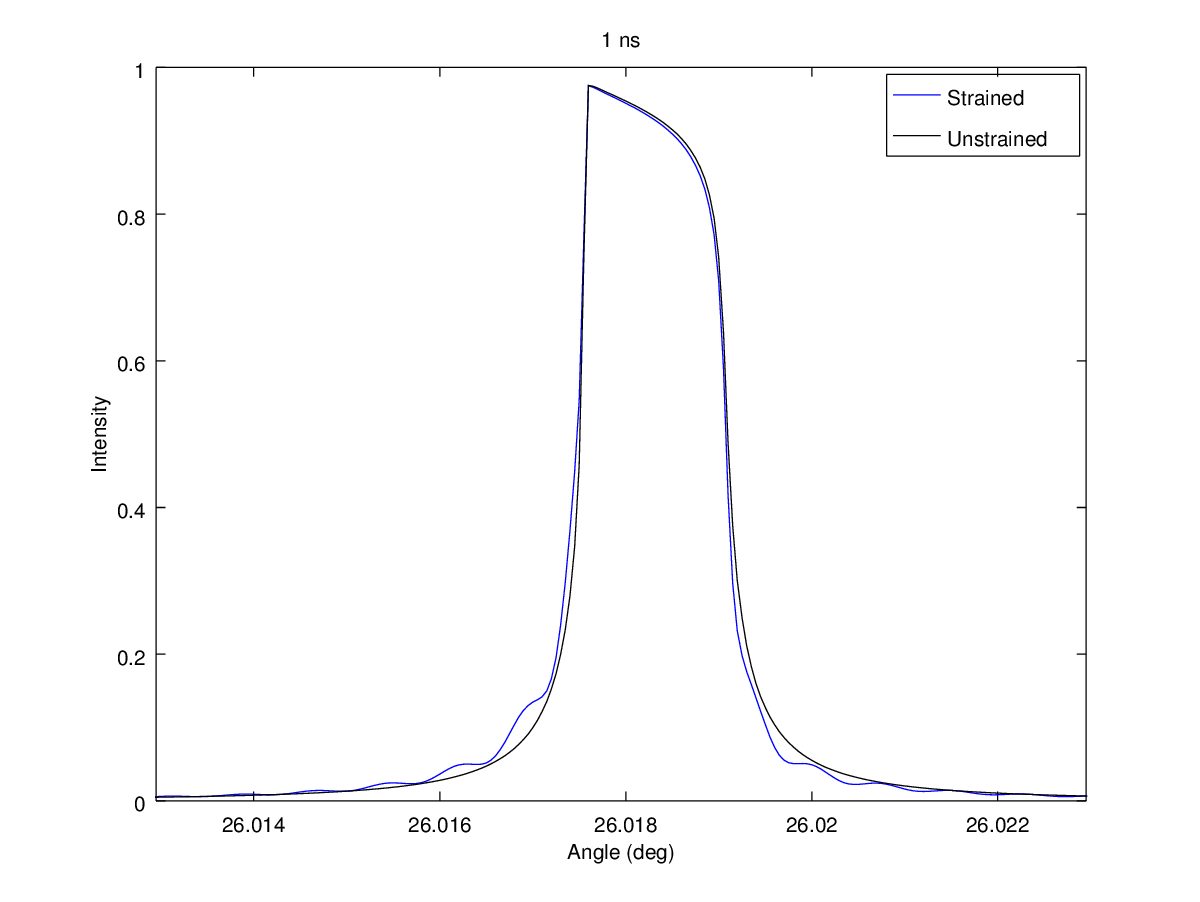
\includegraphics[scale=0.65]{1ns_lin.png}
\caption{External file, 1 ns rocking curve (linear scale).}
\label{fig:1ns_lin}
\end{centering}
\end{figure}

\begin{figure}
\begin{centering}
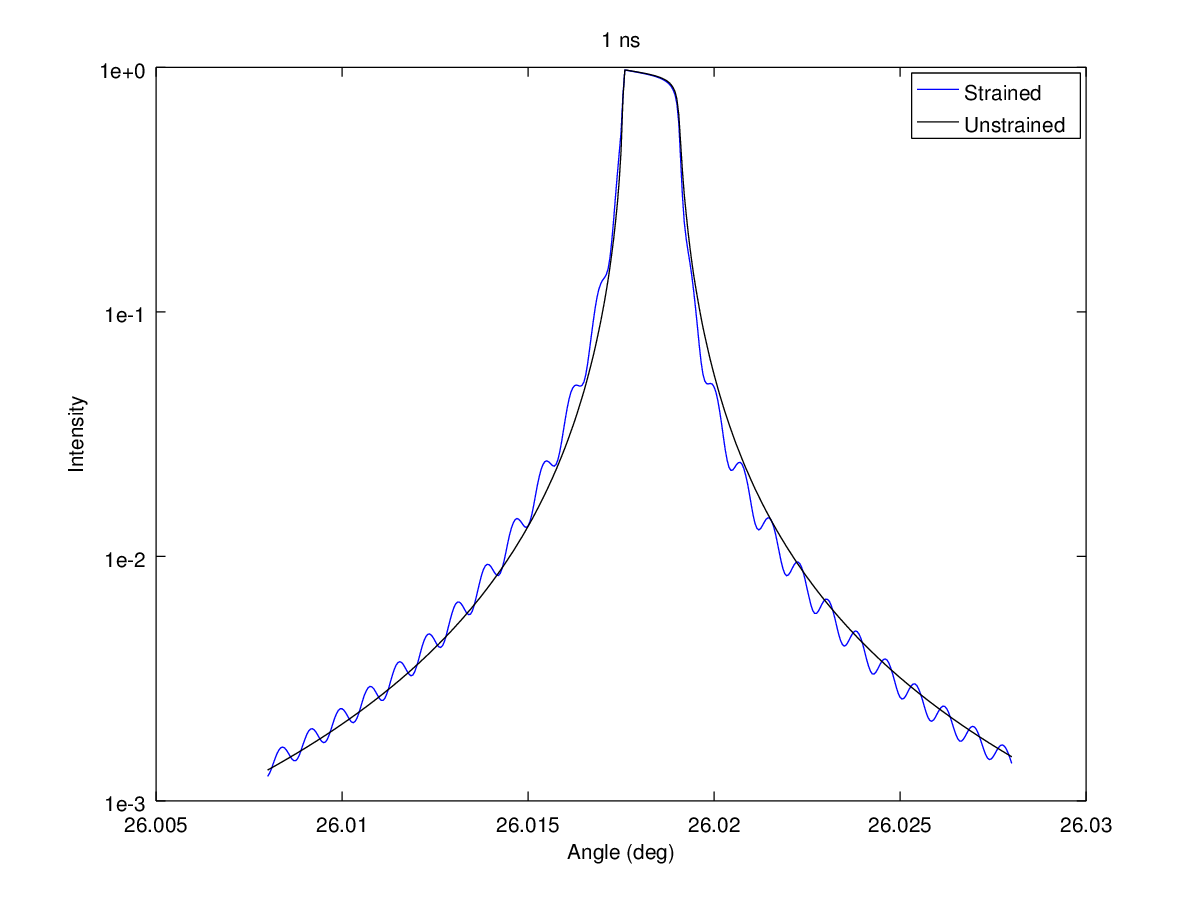
\includegraphics[scale=0.65]{1ns_log.png}
\caption{External file, 1 ns rocking curve (logarithmic scale).}
\label{fig:1ns_log}
\end{centering}
\end{figure}

This analysis is repeated for a 1 ns time delay, and is shown in Figs. \ref{fig:1ns_strain}, \ref{fig:1ns_lin}, and \ref{fig:1ns_log}. The fringes are closer together, indicating that the sharp impulsive strain wave is farther from the surface.  The fringe spacing is now only 0.8 mdeg, corresponding to 4.6 $\mu m$, in agreement with the 1 ns strain profile shown in Fig. \ref{fig:1ns_strain}.  However, as expected, the average strain is about the same as at 400 ps.  The code produces the following output:  

\medskip
\noindent
\texttt{The centroid shift is -0.079 mdeg or -1.4e-06 radians.
For GaAs 0 0 4 at 10.0 keV the estimated average strain is 2.8e-06 .}
\medskip

Although not shown here, the average strain value remains very similar at the end of this particular run (about 2 ns) although the fringes disappear as the impulsive wave moves out of the x-ray probe depth.  It should be noted that actual experimental observation of these very finely strutured fringes would likely be impossible due to finite angular and temporal resolution, which are not taken into account using this method.

\newpage

\subsection{Thermal film model}
Please see the associated documents in \texttt{/strain\_functions/thermalFilmdocs/}.

\section*{Appendix: Code}

The most recent and up to date code should be obtained from \url{https://github.com/elandahl/dynamical-diffraction/tree/TRXD/strain_functions}.  

%This code listing is for reference only. 
 
% \verbatiminput{../thermalFilm.m}

\end{document}
